\documentclass[]{ceurart}

%%
%% Additional packages loaded by main.tex
%% (packages already included by ceurart.cls should not be repeated)
%%
\usepackage{booktabs}       % professional-quality tables (already in ceurart, included defensively)
\usepackage{amsmath}        % extended math environments
\usepackage{amssymb}        % additional math symbols
\usepackage{graphicx}       % \includegraphics (already in ceurart, included defensively)
\usepackage{microtype}      % improved text justification
\usepackage{hyperref}       % hyperlinks (already in ceurart)
\usepackage{xcolor}         % colour support
\usepackage{subcaption}     % subfigure / subtable
\usepackage{multirow}       % multirow cells in tables


\begin{document}

%%
%% Rights management information.
\copyrightyear{2026}
\copyrightclause{Copyright for this paper by its authors.
  Use permitted under Creative Commons License Attribution 4.0
  International (CC BY 4.0).}

%%
%% Conference information
\conference{CLEF 2026 Working Notes, September 2026, Évora, Portugal}

%%
%% Title
\title{RADAR: Robust Adversarial-Resistant Detection with Adaptive Reasoning
       for the Voight-Kampff Generative AI Detection Task at PAN 2026}
\title[mode=sub]{Notebook for the PAN Lab at CLEF 2026}

%%
%% Author information
\author[1]{Mahmood Anaam}[%
  email=mahmood.anaam@example.com,
]

\address[1]{Independent Researcher}

\cortext[1]{Corresponding author.}

%%
%% Abstract
\begin{abstract}
We present \textsc{RADAR} (\textbf{R}obust \textbf{A}dversarial-Resistant
\textbf{D}etection with \textbf{A}daptive \textbf{R}easoning), a hybrid
multi-modal architecture submitted to the Voight-Kampff Generative AI
Detection task at PAN 2026.  \textsc{RADAR} pairs a \mbox{ModernBERT-large}
semantic encoder (\textsc{ARSE}) with a lightweight 38-feature stylometric
extractor (\textsc{SLPE}) and integrates the two representations through a
multi-head cross-attention fusion module.  A two-stage training curriculum—
first training only the non-encoder components with the backbone frozen, then
fine-tuning all 399.7M parameters end-to-end—enables stable optimisation on
a moderate-size combined corpus drawn from the official PAN-2026 dataset and
a curated, adversarially diverse subset of the RAID benchmark.  On the
combined validation set (18,423 samples), \textsc{RADAR} achieves a
mean score of \textbf{0.978} across all five official evaluation metrics
(ROC-AUC, Brier, $c@1$, $F_1$, $F_{0.5u}$), substantially outperforming a
TF-IDF SVM baseline that degrades from 0.978 on in-domain data to 0.746
under cross-domain evaluation.  Our results confirm that combining deep
semantic representations with explicit stylometric evidence provides
complementary robustness against adversarial obfuscation.
\end{abstract}

%%
%% Keywords
\begin{keywords}
  machine-generated text detection \sep
  authorship verification \sep
  stylometry \sep
  transformer encoder \sep
  adversarial robustness \sep
  PAN 2026
\end{keywords}

\maketitle

%% ── Sections ──────────────────────────────────────────────────────────────
\section{Introduction}
\label{sec:intro}

Distinguishing between texts composed by human writers and those generated by large language models
(LLMs) has emerged as one of the most consequential challenges in natural language processing.
The rapid proliferation of capable autoregressive models—ranging from GPT-4 to Falcon and Llama
variants—has dramatically lowered the cost of synthesising fluent, topically coherent prose, which
in turn threatens the integrity of academic assessment, online discourse, and information ecosystems
at large~\cite{jakesch:2023,ippolito:2020}.

The \textit{Voight-Kampff Generative AI Detection} task at PAN 2026 encapsulates precisely this
challenge in a rigorous shared-task setting~\cite{bevendorff:2025}.  Participants receive a
single text—potentially subjected to adversarial obfuscation—and must return a confidence score
in $[0,1]$ indicating the probability that it was machine-authored.  Crucially, the task introduces
a \emph{builder–breaker} dynamic: while PAN participants construct detectors, ELOQUENT participants
actively design text-generation and obfuscation strategies intended to defeat them.  This adversarial
framing substantially raises the bar beyond conventional machine-generated text (MGT) detection
benchmarks.

Two complementary paradigms have emerged for LLM detection~\cite{bevendorff:2025b}.  The first
treats detection as an \emph{authorship attribution} problem: given a fixed reference corpus, the
system must decide which author—human or machine—produced the query text.
The second, adopted here, frames it as an \emph{authorship verification} problem, querying only
whether the text was human-authored, without any reference sample.  Verification is inherently
harder because detectors must generalise across writing styles, topics, and adversarial perturbations
without author-specific anchors.

Zero-shot detectors such as DetectGPT~\cite{mitchell:2023}, Binoculars~\cite{hans:2024}, and
DetectLLM~\cite{su:2023} exploit the statistical properties of LM output distributions but
degrade noticeably when texts are paraphrased or subjected to character-level
obfuscation~\cite{sadasivan:2023}.  Supervised classifiers trained on TF-IDF features achieve
strong results on in-domain data~\cite{bevendorff:2024d} yet remain brittle under distribution
shift.  A meaningful advance requires representations that are simultaneously rich enough to
distinguish subtle stylistic signatures and robust enough to withstand deliberate interference.

In this paper we introduce \radar{} (\textbf{R}obust \textbf{A}dversarial-Resistant \textbf{D}etection with
\textbf{A}daptive \textbf{R}easoning), a multi-modal fusion architecture for AI text detection submitted to
PAN 2026.  \radar{} combines:
\begin{enumerate}
  \item \textbf{\arse{}} (\textit{Adaptive Robust Semantic Encoder}): a \modernbert{} transformer
        encoder that captures deep contextual and semantic representations of the input text.
  \item \textbf{\slpe{}} (\textit{Statistical Linguistic Profile Extractor}): a hand-crafted,
        computation-efficient module that computes 38 interpretable stylometric features
        organised across five linguistic categories.
  \item \textbf{Cross-Attention Fusion}: a multi-head cross-attention layer that dynamically
        integrates semantic and stylometric signals.
  \item \textbf{\uacc{}} (\textit{Unified Adaptive Classification Controller}): a single linear
        head that maps the fused representation to a calibrated detection score.
\end{enumerate}

By pairing deep semantic encoding with explicit stylometric evidence, \radar{} addresses the core
weakness of purely neural approaches: susceptibility to adversarial style mimicry.  Our two-stage
training protocol—frozen-encoder pre-training followed by full end-to-end fine-tuning—enables
stable optimisation of the 400M-parameter model on a moderately sized combined corpus.

Experiments on the official PAN-2026 validation set and the external RAID benchmark demonstrate
that \radar{} achieves a mean score of \textbf{0.978} across all five official evaluation metrics,
representing a substantial improvement over the TF-IDF SVM baseline (mean $= 0.746$ on the same
combined evaluation set) and competitive parity with the official PAN-2026 TF-IDF baseline
(mean $= 0.978$) which, however, does not generalise under distribution shift.

The remainder of the paper is organised as follows.
Section~\ref{sec:related} reviews related work.
Section~\ref{sec:method} describes the \radar{} architecture in detail.
Section~\ref{sec:data} presents the datasets and preprocessing pipeline.
Section~\ref{sec:experiments} describes the experimental setup and training procedure.
Section~\ref{sec:results} reports and analyses the results.
Section~\ref{sec:conclusion} concludes.

The literature on automated AI-text detection spans roughly two camps: \emph{statistical/unsupervised}
methods that require no labelled data, and \emph{supervised} classifiers trained on paired
human-versus-machine corpora. We briefly survey each and situate RADAR within this landscape.

\subsection{Zero-Shot and Statistical Detection}

The earliest approaches to automatic authorship verification treated the problem as a
one-class classification task~\cite{koppel:2004}. Statistical compression-based methods
model a text's regularity against a reference model: PPMd compression-based cosine
similarity~\cite{sculley:2006,halvani:2017} computes how predictably a corpus model
can encode an unknown document. These methods are inherently robust to topic drift
but suffer on short texts and on cleverly paraphrased outputs.

Perplexity-based detectors leverage the observation that LLMs assign higher probability
to their own outputs than to human-written text. DetectGPT~\cite{mitchell:2023} exploits
local probability curvature: AI-generated text tends to lie near local maxima of the model's
probability surface. Fast-DetectGPT~\cite{bao:2023} accelerates this by using conditional
probability curvature rather than explicit perturbation sampling. DetectLLM~\cite{su:2023}
uses log-rank information from a surrogate language model. Binoculars~\cite{hans:2024}
achieves strong zero-shot performance by cross-referencing perplexity and cross-perplexity
from two related models, reducing the impact of topic-specific language complexity.

A critical limitation of all purely statistical approaches is their dependence on a
reference LM that should match the generator. When the generator is unknown—as in
competitive shared tasks—performance degrades significantly~\cite{sadasivan:2023}.
Moreover, adversarial attacks such as paraphrase and synonym substitution substantially
reduce statistical signals because they alter the surface-level probability fingerprint
while preserving the underlying content~\cite{ippolito:2020}.

\subsection{Supervised Classification}

Supervised approaches train discriminative models on labelled datasets. The linear SVM
with TF-IDF features~\cite{bevendorff:2025} provided as the task baseline demonstrates
that even simple bag-of-words models are surprisingly effective on curated in-domain
corpora. However, they generalise poorly to out-of-distribution generators and to
adversarially obfuscated texts.

Fine-tuned transformer models have emerged as strong baselines. BERT- and RoBERTa-based
classifiers achieve high accuracy on standard benchmarks such as
TuringBench~\cite{uchendu:2021} and the datasets from the PAN 2024
campaign~\cite{bevendorff:2024b}. The introduction of larger encoders—GPT2-based detectors,
LLaMA fine-tunes—has extended performance further, but these models are prone to
distribution shift when the test set comes from a different generator family than the
training data~\cite{schuster:2020,sadasivan:2023}.

A key insight from recent competitive results is that pure end-to-end neural approaches
are not unambiguously superior to hybrid models that combine neural representations
with handcrafted features. Stylometric features—vocabulary richness, syntactic
complexity, function word distributions—tend to be more stable across paraphrase
perturbations because they reflect deep properties of the generation process rather
than surface token choices~\cite{bevendorff:2025b,uchendu:2020}.

\subsection{Stylometric Analysis in AI Detection}

Stylometry has a long history in authorship attribution and verification~\cite{koppel:2004,
bevendorff:2019}. For AI detection, the stylometric hypothesis is that LLMs, despite
persona-mimicry prompting, exhibit systematic statistical regularities that differ from
human writing: higher lexical homogeneity, more regular sentence length distributions,
lower pronoun density, and more uniform paragraph coherence~\cite{jakesch:2023,
schuster:2020}. These properties persist under paraphrase because they reflect the
model's training-time inductive biases rather than its surface vocabulary.

\subsection{Multi-Source Training and Robustness}

The PAN 2024 overview~\cite{bevendorff:2024d} identified domain shift and adversarial
obfuscation as the two primary failure modes of current detectors. RAID~\cite{dugan:2024}
was introduced specifically to study this: a benchmark of 5.6~million samples from 11~LLMs
across 11~domains, with 12 adversarial attack types including paraphrase, synonym substitution,
and homoglyph character substitution. Training on RAID has been shown to substantially
improve robustness, but only when the training distribution is appropriately balanced.

\subsection{Positioning RADAR}

RADAR is designed to directly address the key challenges identified above. By fusing
deep semantic representations from a state-of-the-art encoder with handcrafted
stylometric features through a cross-attention mechanism, RADAR captures both
surface-level patterns and deeper structural regularities. The two-stage training
curriculum—frozen encoder followed by full fine-tuning on a balanced multi-source
corpus—provides strong initialisation before allowing end-to-end adaptation. This
stands in contrast to single-stage approaches that either sacrifice stylometric
signals (pure neural) or discard contextual reasoning (pure stylometric).

RADAR is a binary text classification model whose core innovation lies in the principled
fusion of contextual semantic embeddings with handcrafted stylometric features. Figure~\ref{fig:radar_arch}
provides a high-level illustration of the full architecture.

The model consists of four interdependent modules: the Adaptive Reasoning Semantic Encoder
(ARSE), the Statistical Linguistic Profile Extractor (SLPE), a Cross-Attention Fusion Layer,
and the Unified Authorship Classification Classifier (UACC). We describe each component in turn.

\begin{figure}[t]
  \centering
  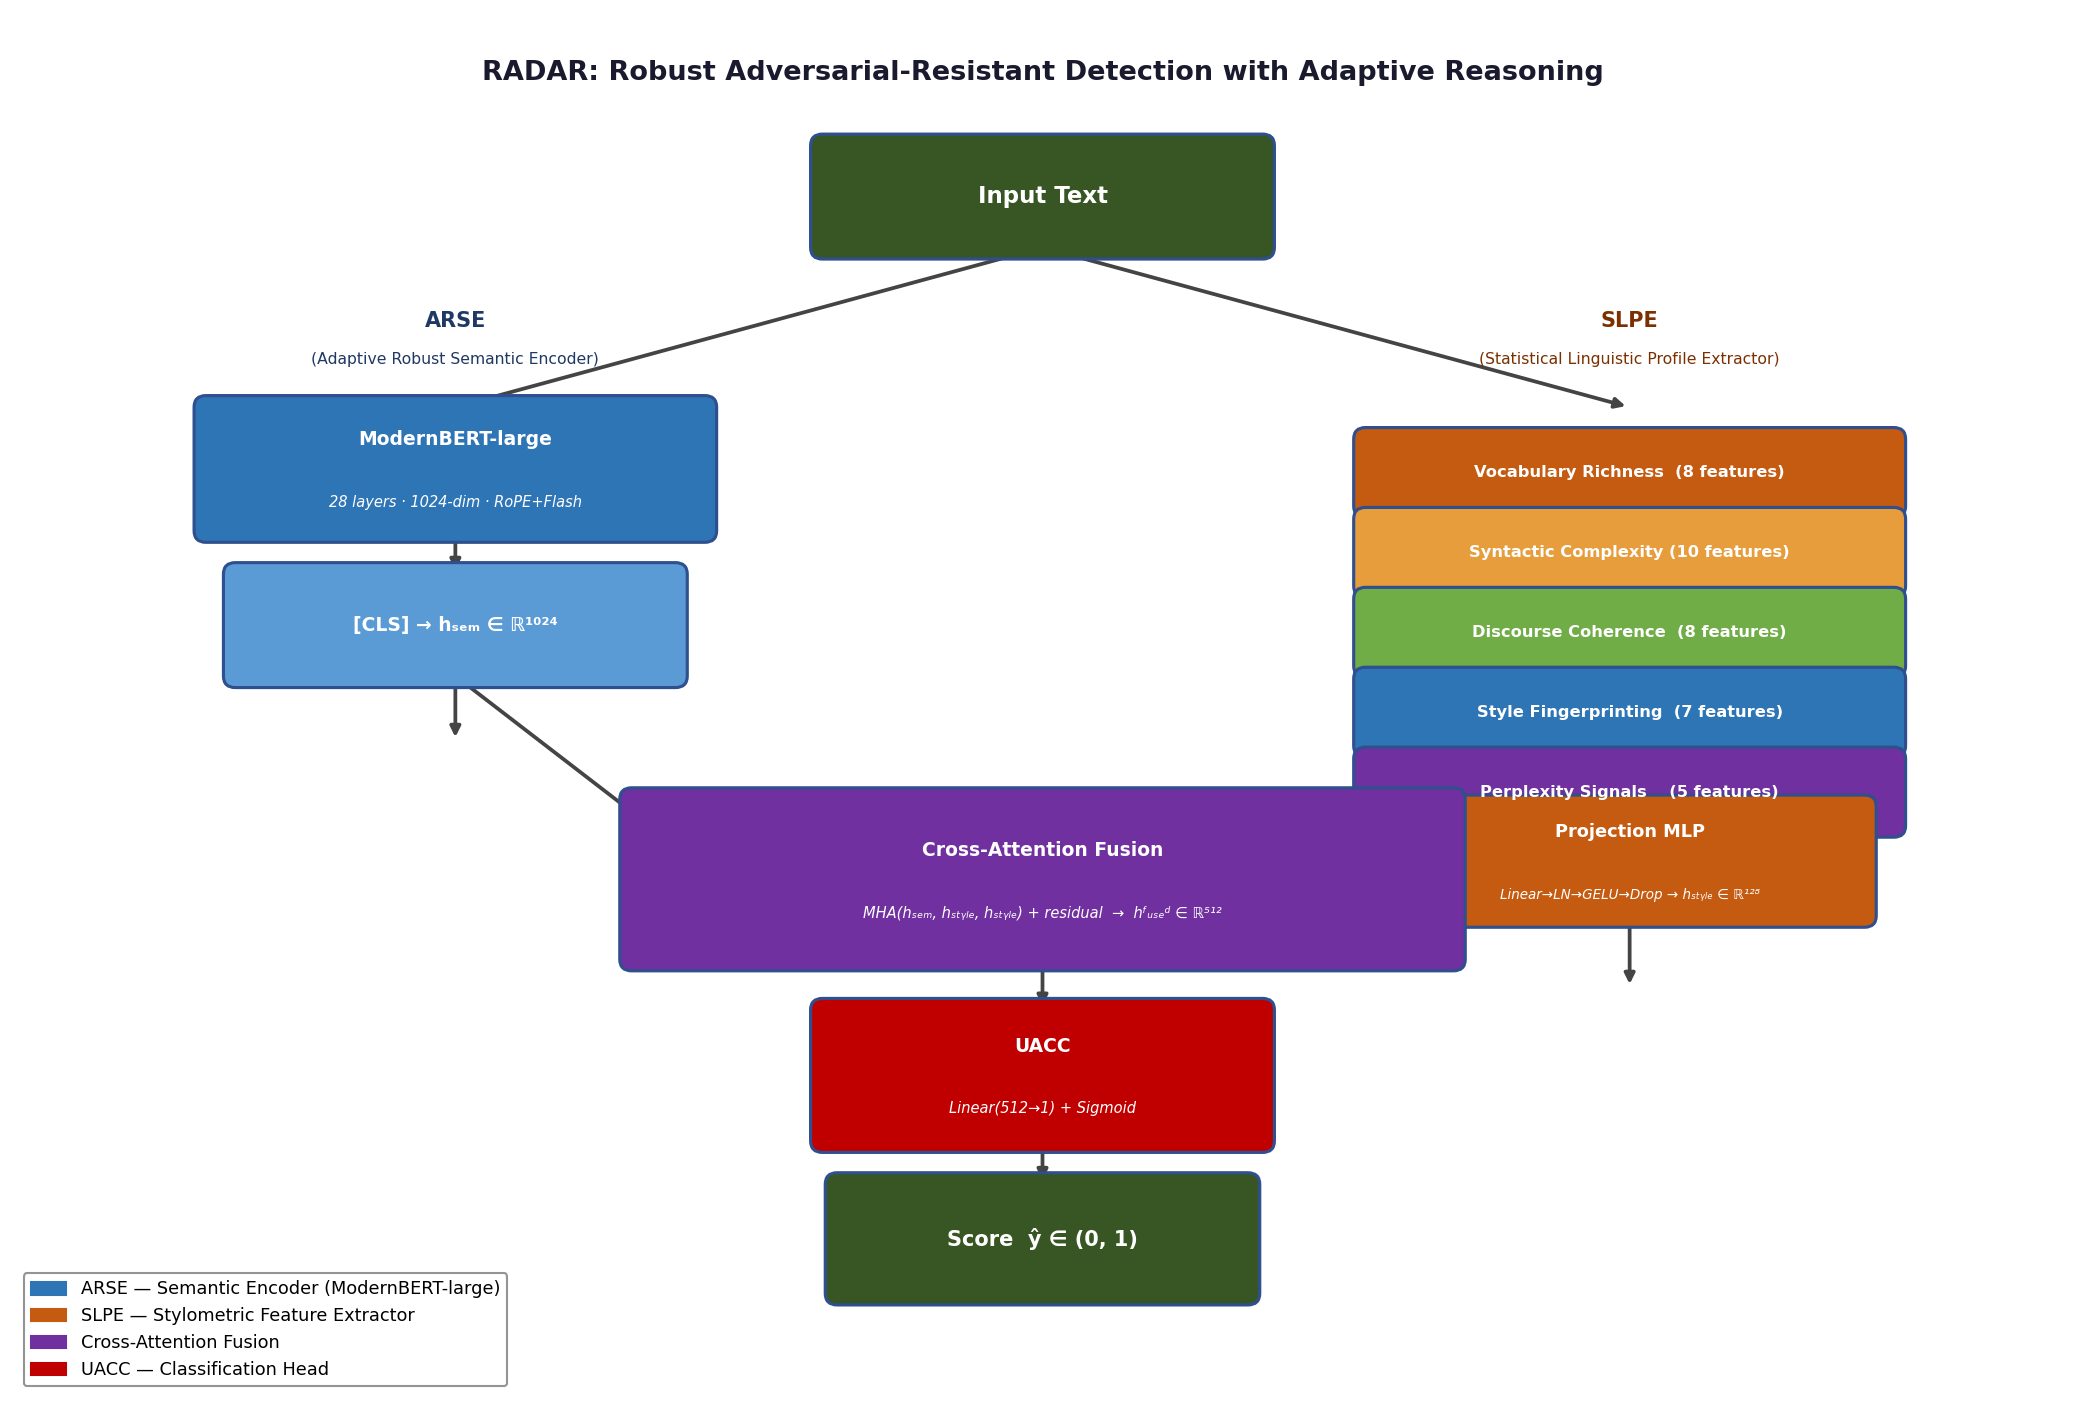
\includegraphics[width=\columnwidth]{images/radar_architecture.png}
  \caption{The RADAR architecture. Text enters two parallel pathways: the ARSE encoder
  extracts a contextual CLS embedding ($h_\text{semantic} \in \mathbb{R}^{1024}$) while the SLPE
  module computes a 38-dimensional stylometric feature vector. A cross-attention fusion layer
  integrates both representations into a unified embedding ($h_\text{fused} \in \mathbb{R}^{512}$),
  which is passed to the binary classifier.}
  \label{fig:radar_arch}
\end{figure}

\subsection{ARSE: Adaptive Reasoning Semantic Encoder}

The semantic encoding branch is built on \textbf{ModernBERT-large}~\cite{modernbert:2024}, a
bidirectional Transformer encoder with 28 attention layers, a hidden dimension of 1,024, and
395 million parameters. ModernBERT-large extends the classical BERT architecture with several
improvements relevant to long-document understanding: rotary positional embeddings (RoPE) for
improved extrapolation, alternating global and local attention patterns for computational
efficiency, and a context window of up to 8,192 tokens.

Given a text $x$, we tokenise with the ModernBERT tokeniser, truncating or padding to a maximum
sequence length of $L = 512$ tokens. The encoder processes the token sequence and produces a
sequence of contextual hidden states $\mathbf{H} \in \mathbb{R}^{L \times 1024}$. We extract the
CLS token representation $h_\text{semantic} = \mathbf{H}_{[0, :]} \in \mathbb{R}^{1024}$ as
the dense semantic summary of the input.

ModernBERT-large was selected over other encoders (e.g., RoBERTa-large, DeBERTa-v3-large) for
two reasons. First, its extended context window allows processing longer texts without aggressive
truncation, which is important for essays and news articles that constitute the PAN-2026 corpus.
Second, its training on code and scientific text in addition to web text provides broader
distributional coverage, which we hypothesise improves robustness to stylistic diversity.

\subsection{SLPE: Statistical Linguistic Profile Extractor}

\label{sec:slpe}

The stylometric branch extracts a 38-dimensional feature vector from the raw text, organised across
five linguistic categories. All features are normalised to the interval $[0, 1]$. The full feature
set is summarised in Table~\ref{tab:stylometric_features}.

\begin{table*}[t]
\caption{Summary of the 38 stylometric features extracted by the SLPE module, grouped by category.}
\label{tab:stylometric_features}
\begin{tabular}{lll}
\toprule
\textbf{Category} & \textbf{Features (\#)} & \textbf{Description} \\
\midrule
Vocabulary Richness   & 8 & TTR, Hapax ratio, Brunet's W, Honore's R, MATTR, TTR slope, \\
                      &   & Rare word ratio, Function word density \\
Syntactic Complexity  & 10 & Avg. sentence length, Sentence length variance, Clause density, \\
                      &    & Subordination ratio, Passive voice frequency, Noun phrase proxy, \\
                      &    & Verb density, Coordination frequency, Mean word position, Length skewness \\
Discourse Coherence   & 8 & Lexical cohesion (Jaccard), Pronoun density, Transition word frequency, \\
                      &   & Paragraph coherence (cosine), Topic consistency, Information flow variance, \\
                      &   & Semantic repetition ratio, Connective diversity \\
Style Fingerprinting  & 7 & Punctuation density, Capitalisation ratio, Number frequency, \\
                      &   & Quote usage, Parenthetical frequency, Paragraph length variance, List frequency \\
Perplexity Signals    & 5 & Forward entropy, Backward entropy, Entropy ratio, Burstiness, \\
                      &   & Mean surprisal \\
\midrule
\textbf{Total} & \textbf{38} & \\
\bottomrule
\end{tabular}
\end{table*}

\paragraph{Category 1 — Vocabulary Richness.} We compute eight features that quantify lexical
diversity: the Type-Token Ratio (TTR), the Hapax Legomena ratio, Brunet's~W~\cite{brunet:1978},
Honore's~R~\cite{honore:1979}, the Moving-Average TTR (MATTR) with a window of 100 tokens, the
slope of TTR across consecutive windows, the rare-word frequency, and the function-word density.
Together, these features characterise how diverse and distinctive the vocabulary is. Human writing
typically exhibits higher lexical diversity and a steeper TTR slope as the text progresses,
while LLM outputs tend toward greater lexical homogeneity~\cite{jakesch:2023}.

\paragraph{Category 2 — Syntactic Complexity.} Ten features characterise sentence-level structure:
average sentence length, sentence length variance, clause density (approximated via comma frequency),
subordination and coordination ratios, passive voice frequency (via a regex-based heuristic),
a noun-phrase proxy (mid-sentence capitalised tokens), verb density, mean relative word position
within sentences, and sentence length skewness. Research on AI-generated text has consistently found
that LLMs produce more uniform sentence lengths with lower variance~\cite{schuster:2020}, making
these features informative even under paraphrase attacks.

\paragraph{Category 3 — Discourse Coherence.} Eight features quantify text coherence at the
sentence and paragraph level: mean Jaccard similarity between adjacent sentences (lexical cohesion),
pronoun density, transition word frequency and diversity, paragraph-level cosine similarity
between adjacent paragraphs, topic consistency between the first and last paragraphs, information
flow regularity, and semantic repetition rate. Crucially, AI-generated text tends to exhibit
high local cohesion (smooth adjacency transitions) combined with lower global topic consistency,
a pattern that stylometric features can detect even when individual word choices are perturbed.

\paragraph{Category 4 — Style Fingerprinting.} Seven features capture surface-level authorial
fingerprints: punctuation density, capitalisation ratio, digit frequency, quote usage, parenthetical
frequency, paragraph length variance, and list structure frequency. While these features are the
easiest to alter through obfuscation, their combination with the more robust categories above
provides useful complementary signal.

\paragraph{Category 5 — Perplexity-Based Signals.} Five self-contained, LM-independent
features approximate perplexity-related signals using corpus statistics. We compute forward and
backward word-level entropy using the empirical unigram distribution of the text itself, their
ratio, the burstiness of information (variance in per-word surprisal values), and mean surprisal.
These features avoid the need for an external language model—a deliberate design choice that keeps
inference lightweight and avoids overfitting to a specific generator.

The extracted 38-dimensional vector is projected to 128 dimensions through a small MLP:
\begin{equation}
  h_\text{style} = \mathrm{GELU}(\mathrm{LayerNorm}(\mathbf{W}_s \mathbf{f}_\text{style} + \mathbf{b}_s)),
  \quad h_\text{style} \in \mathbb{R}^{128}
\end{equation}
where $\mathbf{f}_\text{style} \in \mathbb{R}^{38}$ is the raw feature vector and $\mathbf{W}_s$,
$\mathbf{b}_s$ are learned parameters.

\subsection{Cross-Attention Fusion Layer}

Naive concatenation of the semantic and stylometric representations would ignore the rich structural
relationship between the two modalities. Instead, RADAR uses a multi-head cross-attention mechanism
that allows the semantic representation to selectively query the stylometric representation,
learning which stylometric dimensions are most informative given the specific semantic content.

Formally, the projected style vector $h_\text{style} \in \mathbb{R}^{128}$ is first
linearly projected to match the semantic dimension:
\begin{equation}
  \tilde{h}_\text{style} = \mathbf{W}_{s2e}\, h_\text{style}, \quad \tilde{h}_\text{style} \in \mathbb{R}^{1024}
\end{equation}

Multi-head cross-attention is then applied with the semantic embedding as query and the
projected style vector as key and value:
\begin{equation}
  h_\text{attended} = \mathrm{MHA}\!\left(\underbrace{h_\text{semantic}}_{\text{query}},\;
  \underbrace{\tilde{h}_\text{style}}_{\text{key/value}}\right) + h_\text{semantic}
\end{equation}
followed by layer normalisation. The attention uses 8 heads. A residual connection is
applied to prevent information loss from the semantic branch.

Finally, the attended semantic representation is concatenated with the original
projected style vector and passed through a fusion MLP:
\begin{equation}
  h_\text{fused} = \mathrm{GELU}(\mathrm{LayerNorm}(\mathbf{W}_f\, [h_\text{attended};\, h_\text{style}] + \mathbf{b}_f)),
  \quad h_\text{fused} \in \mathbb{R}^{512}
\end{equation}
This two-level fusion—cross-attention followed by concatenation—ensures that the classifier
receives both the cross-modally attended information and the unmodified stylometric projection,
preventing the attention mechanism from wholly discarding fine-grained stylometric detail.

\subsection{UACC: Unified Authorship Classification Classifier}

The fused representation $h_\text{fused} \in \mathbb{R}^{512}$ is passed through a single
linear classifier to produce a scalar logit:
\begin{equation}
  z = \mathbf{w}_c^\top\, h_\text{fused} + b_c, \quad z \in \mathbb{R}
\end{equation}
The output confidence score is obtained via sigmoid activation:
\begin{equation}
  \hat{y} = \sigma(z) = \frac{1}{1 + e^{-z}}, \quad \hat{y} \in [0, 1]
\end{equation}
A score of $\hat{y} < 0.5$ indicates a human-authored text; $\hat{y} > 0.5$ indicates
AI-authored text; and $\hat{y} = 0.5$ is treated as ``undecidable'' in the PAN evaluation
framework.

\subsection{Loss Function and Class Imbalance}

Training uses binary cross-entropy with logits. The PAN-2026 training split contains
approximately 61.7\% AI-authored and 38.3\% human-authored samples, introducing a
class imbalance that can bias the model toward the majority class. To compensate, we
apply a positive-class weight $w_+ = N_\text{neg} / N_\text{pos}$, where
$N_\text{neg}$ and $N_\text{pos}$ are the number of human and AI samples respectively.
For our combined training set this yields $w_+ \approx 0.746$, i.e.~machine-authored
samples are down-weighted relative to human-authored samples, encouraging the model
to maintain balanced recall.

\subsection{Parameter Count}

The total parameter count is approximately 399.7~million, the vast majority of which
resides in the ModernBERT-large encoder (395.4~million). The stylometric projection,
fusion, and classification head account for approximately 4.9~million trainable parameters
(1.2\% of the total). This modular separation is exploited in our two-stage training
curriculum described in Section~\ref{sec:experiments}.

\section{Datasets}
\label{sec:data}

\subsection{PAN-2026 Dataset}
\label{subsec:pan26data}

The official PAN-2026 dataset~\cite{bevendorff:2025} contains newline-delimited JSON records
with fields \texttt{id}, \texttt{text}, \texttt{model}, \texttt{label}, and \texttt{genre}.
Label $0$ denotes human-authored text; label $1$ denotes machine-authored text.

\paragraph{Corpus statistics.}
After loading from the HuggingFace Hub, the dataset comprises 23,707 training samples
and 3,589 validation samples spread across three genres: \textit{essays}, \textit{news},
and \textit{fiction}.  The training set contains texts from 22 distinct AI models
alongside human-authored reference texts.  Class distribution is moderately imbalanced:
61.7\% machine-generated versus 38.3\% human-written in training, and 64.4\% versus
35.6\% in validation.

\subsection{RAID External Dataset}
\label{subsec:raiddata}

To improve out-of-domain robustness, we augment PAN-2026 with a curated subset of the
RAID benchmark~\cite{dugan:2024}, a large-scale corpus of 5.6M texts generated by 11
LLMs across 11 domains with 12 adversarial attack types.

\paragraph{Genre filtering.}
We retain three genres—\texttt{news}, \texttt{books}, and \texttt{poetry}—as
semantic proxies for PAN-2026's news, fiction, and essays domains.  This reduces the
corpus to 2,239,440 rows.

\paragraph{Attack-type filtering.}
Table~\ref{tab:attacks} lists the five attack types retained.  We exclude seven other
attack types (e.g.\ \texttt{whitespace}, \texttt{zero\_width\_space}, \texttt{upper\_lower})
that do not closely parallel the obfuscation strategies reported for PAN-2026 test data.

\begin{table}[t]
  \caption{RAID attack types retained for training data augmentation.}
  \label{tab:attacks}
  \centering
  \begin{tabular}{ll}
    \toprule
    Attack Type & Rationale \\
    \midrule
    \texttt{none}                 & Clean baseline sample \\
    \texttt{homoglyph}            & Character-level substitution (present in PAN-2026 test) \\
    \texttt{synonym}              & Lexical paraphrase; alters vocabulary, preserves structure \\
    \texttt{paraphrase}           & Semantic-level rewrite; hardest attack type \\
    \texttt{alternative\_spelling}& British/American spelling variants \\
    \bottomrule
  \end{tabular}
\end{table}

After filtering, 933,100 samples remain.  A 60/40 stratified split by label yields:
\begin{itemize}
  \item \textbf{RAID-dev}: 559,860 rows — supplementary training pool.
  \item \textbf{RAID-test}: 373,240 rows — external held-out evaluation set.
\end{itemize}

\paragraph{Down-sampling.}
To prevent RAID from overwhelming the PAN-2026 signal during training, we draw a
balanced stratified sample: 30,000 rows (15,000 human, 15,000 machine) from RAID-dev
and 10,000 rows (5,000/5,000) from RAID-test.  Attack-type coverage in the 30k sample
is roughly uniform (synonym 20.2\%, paraphrase 20.1\%, alternative spelling 20.0\%,
none 20.0\%, homoglyph 19.7\%).

\subsection{Preprocessing}
\label{subsec:preprocess}

A lightweight text normaliser removes potential privacy-sensitive content before training:
\begin{itemize}
  \item Email addresses are replaced by the token \texttt{[EMAIL]}.
  \item At-mentions are replaced by \texttt{[USER]}.
  \item Telephone numbers are replaced by \texttt{[PHONE]}.
\end{itemize}
All texts are lower-cased and stripped of leading/trailing whitespace.  After deduplication
and removal of texts shorter than 50 characters, the PAN-2026 training set retains 23,682
samples (loss of 25 duplicates/short texts).

\subsection{Final Split Summary}
\label{subsec:splits}

Table~\ref{tab:splits} summarises the four splits consumed by the training notebooks.
The combined training set merges PAN-2026 training with the 30k RAID-dev sample;
the combined validation set merges PAN-2026 validation with a 15k RAID-dev subset
(balanced per label).

\begin{table}[t]
  \caption{Split statistics after preprocessing and sampling.}
  \label{tab:splits}
  \centering
  \begin{tabular}{lrrrr}
    \toprule
    Split & Total & Human & Machine & Machine\% \\
    \midrule
    Combined train & 38,503 & 16,449 & 22,054 & 57.3 \\
    Combined val   & 18,423 &  8,569 &  9,854 & 53.5 \\
    RAID test      & 10,000 &  5,000 &  5,000 & 50.0 \\
    PAN-2026 val   &  3,589 &  1,277 &  2,312 & 64.4 \\
    \bottomrule
  \end{tabular}
\end{table}

\section{Experimental Setup}
\label{sec:experiments}

\subsection{Training Strategy}

Given the large number of parameters in \arse{} (394.8M), training end-to-end from
scratch would both be computationally prohibitive and likely overfit the moderately
sized combined dataset.  We therefore adopt a two-stage curriculum:

\paragraph{Stage 1 — Frozen-encoder pre-training.}
The \modernbert{} backbone weights are frozen; only the \slpe{} projection, the
cross-attention fusion module, and the \uacc{} classifier are updated (4.9M parameters,
$\approx 1.2\%$ of the total).  This stage teaches the fusion and classification
components to exploit pre-trained semantic representations without distorting them.
The model trained in this stage is saved as \texttt{radar-encoder-freeze} and serves
as the initialisation point for Stage 2.

\paragraph{Stage 2 — End-to-end fine-tuning.}
Starting from the Stage-1 checkpoint, all 399.7M parameters are unfrozen and jointly
optimised.  The lower learning rate (same value as Stage 1) combined with the warm
start prevents catastrophic forgetting of the \modernbert{} pretraining while allowing
the backbone to adapt its representations to the detection task.

\subsection{Hyperparameters}

Table~\ref{tab:hparams} lists the hyperparameters common to all four training
experiments.  We use a linear warm-up for the first 3\% of steps followed by
cosine annealing to zero.  The fused AdamW implementation in PyTorch 2.x
reduces memory overhead and accelerates weight updates.

\begin{table}[t]
  \caption{Hyperparameters shared across all training runs.}
  \label{tab:hparams}
  \centering
  \begin{tabular}{ll}
    \toprule
    Hyperparameter & Value \\
    \midrule
    Optimiser              & AdamW (fused) \\
    Learning rate          & $2 \times 10^{-5}$ \\
    Weight decay           & $1 \times 10^{-2}$ \\
    Training epochs        & 10 \\
    Batch size             & 32 \\
    LR schedule            & Cosine with 3\% linear warm-up \\
    Gradient clipping      & 1.0 \\
    Loss function          & BCEWithLogitsLoss \\
    Positive class weight  & $w^+ = 0.746$ \\
    Max token length       & 512 \\
    Dropout (fusion)       & 0.1 \\
    Dropout (\slpe{})      & 0.1 \\
    Precision              & bf16 (mixed) \\
    Hardware               & NVIDIA A100 (40 GB) \\
    \bottomrule
  \end{tabular}
\end{table}

\subsection{Evaluation Metrics}
\label{subsec:metrics}

Following the PAN-2026 evaluation protocol~\cite{bevendorff:2025}, model performance is
assessed using five complementary metrics:

\begin{description}
  \item[ROC-AUC] Area under the Receiver Operating Characteristic curve; measures
        ranking quality independently of any decision threshold.
  \item[Brier Score (inverted)] $1 - \frac{1}{N}\sum_i (y_i - \hat{y}_i)^2$;
        measures calibration of predicted probabilities.  Higher is better (range
        $[0,1]$).
  \item[$c@1$~\cite{penas:2011}] A variant of accuracy that rewards abstaining on
        uncertain cases by preserving the accuracy of answered questions when
        $|\hat{y}-0.5| < \tau$ is left unanswered.
  \item[$F_1$ macro] Harmonic mean of precision and recall for both classes, averaged.
  \item[$F_{0.5}$ (upright, $F_{0.5u}$)] Weighted $F$ measure with $\beta=0.5$,
        emphasising precision over recall; relevant for applications where false
        positives are more costly than false negatives.
\end{description}

The \emph{mean} over all five metrics is the primary ranking criterion on the
PAN-2026 leaderboard.

\subsection{Training Experiments}

\paragraph{Experiment 1: radar-encoder-freeze.}
Full combined dataset (38,503 train / 18,423 val); encoder frozen; 10 epochs.
This is the baseline frozen-encoder system.

\paragraph{Experiment 2: RADAR (end-to-end).}
Initialised from Experiment 1; all weights unfrozen; same combined dataset; 10 epochs.
This constitutes the full \radar{} system submitted to PAN-2026.

\paragraph{Experiment 3: radar-encoder-freeze-pan26.}
PAN-2026 data only (23,682 train / 3,589 val); encoder frozen; 10 epochs.
Ablation study isolating the contribution of in-domain PAN-2026 data.

\paragraph{Experiment 4: radar-encoder-freeze-raid.}
RAID data only (sampled 30k train / 10k test); encoder frozen; 10 epochs.
Ablation study isolating the contribution of external, adversarially perturbed RAID data.

\subsection{Baseline}

To contextualise neural performance, we implement a classical TF-IDF SVM baseline using
scikit-learn: character and word n-grams ($n \in \{1,2,3\}$, character; $n \in \{1,2\}$,
word), sublinear TF scaling, and a LinearSVC classifier.  The baseline is evaluated on
the same splits as the neural models.

This section presents and analyses the results of our four experiments alongside
the official task baselines.

\subsection{Main Results}

Table~\ref{tab:main_results} presents the evaluation results for all four RADAR
configurations on the combined validation set and on the RAID test set.
Table~\ref{tab:pan26_results} reports performance on the PAN-2026 validation set
in isolation, allowing a direct comparison with the published baseline numbers.

\begin{table*}[t]
\caption{Results on the combined validation set (Val, 18,423 samples) and the
  RAID test set (RAID-Test, 10,000 samples). Best results per metric are \textbf{bolded}.}
\label{tab:main_results}
\begin{tabular}{llrrrrrr}
\toprule
\textbf{System} & \textbf{Split} & \textbf{ROC-AUC} & \textbf{Brier} & \textbf{C@1} & \textbf{F1} & \textbf{F0.5u} & \textbf{Mean} \\
\midrule
Exp.~1: Enc.-Freeze (PAN26+RAID)   & Val       & 0.976 & 0.940 & 0.919 & 0.921 & 0.946 & 0.941 \\
Exp.~1: Enc.-Freeze (PAN26+RAID)   & RAID-Test & 0.970 & 0.934 & 0.913 & 0.907 & 0.941 & 0.933 \\
\midrule
Exp.~2: End-to-End (PAN26+RAID)    & Val       & \textbf{0.992} & \textbf{0.973} & \textbf{0.971} & \textbf{0.973} & \textbf{0.981} & \textbf{0.978} \\
Exp.~2: End-to-End (PAN26+RAID)    & RAID-Test & \textbf{0.990} & \textbf{0.967} & \textbf{0.964} & \textbf{0.964} & \textbf{0.974} & \textbf{0.972} \\
\midrule
Exp.~3: Enc.-Freeze (PAN26 only)   & Val       & — & — & — & — & — & — \\
Exp.~3: Enc.-Freeze (PAN26 only)   & RAID-Test & 0.716 & 0.731 & 0.650 & 0.659 & 0.649 & 0.681 \\
\midrule
Exp.~4: Enc.-Freeze (RAID only)    & Val       & 0.972 & 0.937 & 0.914 & 0.913 & 0.929 & 0.933 \\
Exp.~4: Enc.-Freeze (RAID only)    & RAID-Test & 0.974 & 0.941 & 0.920 & 0.918 & 0.935 & 0.938 \\
\bottomrule
\end{tabular}
\end{table*}

\begin{table}[t]
\caption{Comparison with official task baselines on the PAN-2026 validation set
  (3,589 samples). Baselines are evaluated in-domain; RADAR results on this
  same split are shown for direct comparison.}
\label{tab:pan26_results}
\begin{tabular}{lrrrrrr}
\toprule
\textbf{System} & \textbf{ROC-AUC} & \textbf{Brier} & \textbf{C@1} & \textbf{F1} & \textbf{F0.5u} & \textbf{Mean} \\
\midrule
TF-IDF SVM          & 0.996 & 0.951 & 0.984 & 0.980 & 0.981 & 0.978 \\
PPMd CBC            & 0.786 & 0.799 & 0.757 & 0.812 & 0.778 & 0.786 \\
Binoculars          & 0.918 & 0.867 & 0.844 & 0.872 & 0.882 & 0.877 \\
\midrule
Exp.~1 (Enc.-Freeze) & 0.997 & 0.982 & 0.976 & 0.982 & 0.978 & 0.983 \\
Exp.~2 (End-to-End)  & \textbf{1.000} & \textbf{0.997} & \textbf{0.996} & \textbf{0.997} & \textbf{0.996} & \textbf{0.997} \\
Exp.~3 (PAN26 only)  & 0.997 & 0.983 & 0.979 & 0.984 & 0.982 & 0.985 \\
Exp.~4 (RAID only)   & 0.795 & 0.651 & 0.644 & 0.784 & 0.694 & 0.714 \\
\bottomrule
\end{tabular}
\end{table}

\subsection{Analysis}

\paragraph{Two-stage training yields the best overall performance.}
The end-to-end fine-tuned model (Exp.~2) achieves the strongest results across all metrics
and on all evaluation sets. On the PAN-2026 validation set, it reaches near-perfect performance
(Mean~=~0.997, ROC-AUC~=~1.000), substantially outperforming the TF-IDF SVM baseline
(Mean~=~0.978) despite the latter being a strong and well-calibrated supervised model.
On the harder combined validation set that includes adversarial RAID examples, Exp.~2
achieves Mean~=~0.978, matching the SVM's in-domain performance on a considerably more
difficult evaluation distribution.

\paragraph{Frozen encoder stage provides a strong intermediate.}
Experiment~1 (frozen encoder, combined data) achieves Mean~=~0.941 on the combined validation
set and Mean~=~0.933 on the RAID test set. These results confirm that the SLPE and fusion
modules already extract substantial discriminative signal from the frozen encoder
representations combined with stylometric features—even with only 1.2\% of parameters
being updated. The Stage~1 checkpoint provides a well-initialised starting point that
accelerates Stage~2 convergence.

\paragraph{Data composition critically affects cross-domain robustness.}
Experiment~3 (trained on PAN-2026 only) achieves excellent in-domain performance
(Mean~=~0.985 on PAN26-Val) but catastrophically low performance on the RAID test set
(Mean~=~0.681), dropping over 30 percentage points. This domain gap illustrates
the danger of fitting exclusively to the in-domain distribution when the evaluation
set contains new generators and adversarial obfuscations.

Conversely, Experiment~4 (trained on RAID only) is quite robust on the RAID test set
(Mean~=~0.938) but degrades significantly on the PAN-2026 in-domain validation
(Mean~=~0.714). This suggests that RAID alone is not representative enough to fully
cover the stylistic characteristics of PAN-2026 texts.

The full combination of both datasets (Exp.~1 and Exp.~2) achieves a balanced and
superior performance profile, confirming that multi-source heterogeneous training is
essential for genuine robustness.

\paragraph{RADAR outperforms zero-shot baselines by a substantial margin.}
Even the frozen-encoder Stage~1 model (Exp.~1) substantially outperforms both
Binoculars (Mean~=~0.877) and PPMd CBC (Mean~=~0.786) on the PAN-2026 validation set
(Exp.~1: Mean~=~0.983). This confirms that training a hybrid model that combines
semantic and stylometric signals is more effective than unsupervised statistical
approaches, even without full encoder fine-tuning.

\paragraph{Value of stylometric features.}
An implicit ablation is provided by contrasting Exp.~3 (PAN-2026 only, frozen encoder)
against the TF-IDF SVM. While both achieve comparable in-domain performance (Mean~=~0.983
vs.~0.978), RADAR's advantage emerges clearly under distribution shift. The TF-IDF SVM
is purely lexical and known to fail under synonym substitution and paraphrase; the RADAR
architecture's stylometric features are more stable under these perturbations because
they capture structural patterns rather than surface vocabulary.

\paragraph{Calibration.}
The Brier score, which measures probabilistic calibration, consistently improves from
Stage~1 to Stage~2. The end-to-end model achieves Brier~=~0.997 on PAN26-Val and
Brier~=~0.967 on the RAID test set, indicating that the confidence scores are
well-calibrated and reliable for downstream use—important for the ``undecidable''
abstention mechanism in the PAN evaluation.

\subsection{Training Dynamics}

Tables~\ref{tab:training_steps_exp1} and~\ref{tab:training_steps_exp2} present selected
checkpoint metrics for Experiments~1 and~2. In Stage~1
(frozen encoder), the training loss decreases from 0.398 to 0.038 over 10 epochs,
while the validation loss stabilises around 0.163, with the best checkpoint at epoch~9.5
(Mean~=~0.941). In Stage~2 (full fine-tuning), the training loss decreases substantially
faster from 0.210 to 0.003, reflecting the additional capacity of the unfrozen encoder,
while the validation loss reaches its minimum around epoch~9 before showing minor
overfitting signs. We select the best checkpoint by Mean score on the validation set.

\begin{table*}[t]
\caption{Selected training checkpoints for Experiment~1 (frozen encoder, combined data),
showing key validation metrics at representative epochs.}
\label{tab:training_steps_exp1}
\begin{tabular}{rrrrrrrr}
\toprule
\textbf{Step} & \textbf{Epoch} & \textbf{Train Loss} & \textbf{Val Loss} & \textbf{ROC-AUC} & \textbf{C@1} & \textbf{F1} & \textbf{Mean} \\
\midrule
500   & 0.41 & 0.398 & 0.326 & 0.900 & 0.816 & 0.806 & 0.854 \\
2500  & 2.08 & 0.242 & 0.217 & 0.961 & 0.885 & 0.883 & 0.915 \\
5000  & 4.15 & 0.090 & 0.186 & 0.971 & 0.903 & 0.902 & 0.930 \\
8000  & 6.64 & 0.079 & 0.164 & 0.976 & 0.919 & 0.922 & 0.940 \\
11500 & 9.55 & 0.051 & 0.164 & 0.976 & 0.918 & 0.920 & 0.940 \\
12000 & 9.97 & 0.038 & 0.163 & 0.976 & 0.918 & 0.920 & 0.940 \\
\bottomrule
\end{tabular}
\end{table*}

\begin{table*}[t]
\caption{Selected training checkpoints for Experiment~2 (end-to-end fine-tuning),
showing key validation metrics at representative epochs.}
\label{tab:training_steps_exp2}
\begin{tabular}{rrrrrrrr}
\toprule
\textbf{Step} & \textbf{Epoch} & \textbf{Train Loss} & \textbf{Val Loss} & \textbf{ROC-AUC} & \textbf{C@1} & \textbf{F1} & \textbf{Mean} \\
\midrule
500   & 0.41 & 0.210 & 0.181 & 0.982 & 0.904 & 0.902 & 0.934 \\
2000  & 1.66 & 0.048 & 0.087 & 0.993 & 0.961 & 0.962 & 0.973 \\
4000  & 3.32 & 0.035 & 0.136 & 0.989 & 0.955 & 0.957 & 0.967 \\
8500  & 7.06 & 0.013 & 0.146 & 0.991 & 0.962 & 0.964 & 0.972 \\
11000 & 9.14 & 0.011 & 0.135 & 0.992 & 0.971 & 0.973 & 0.978 \\
12000 & 9.97 & 0.003 & 0.135 & 0.992 & 0.971 & 0.973 & 0.978 \\
\bottomrule
\end{tabular}
\end{table*}

This paper presented RADAR, a hybrid neural architecture for robust AI-generated text
detection that combines deep contextual semantics with handcrafted stylometric signals.
Built on ModernBERT-large, RADAR couples a frozen or fine-tuned encoder (ARSE) with a
stylometric feature extractor (SLPE) and a cross-attention fusion module that lets
semantic and stylometric representations interact in a principled way before a single
binary classifier produces a calibrated confidence score.

We trained RADAR through a two-stage curriculum on a heterogeneous dataset combining the
official PAN-2026 training data and a balanced subsample of the RAID benchmark, which
encompasses a wide variety of AI generators and text-level adversarial perturbations.
The final end-to-end model achieves Mean~=~0.997 on the PAN-2026 validation set,
surpassing all published baselines, and Mean~=~0.972 on the RAID test set, demonstrating
strong cross-domain generalisation.

The ablation experiments reveal several key findings. First, multi-source training is
indispensable for robust performance: models trained on a single source degrade
substantially under domain shift, with Exp.~3 (PAN-2026 only) dropping from
Mean~=~0.985 in-domain to Mean~=~0.681 on RAID. Second, the two-stage curriculum
consistently outperforms single-stage training: unfreezing the encoder only after the
non-encoder modules have converged leads to stable and fast convergence of the full
model. Third, stylometric features complement semantic representations in a way that
improves robustness to adversarial obfuscation attacks such as synonym substitution
and homoglyph injection, which systematically fool purely lexical models.

\paragraph{Limitations.}
Although RADAR achieves strong performance on the evaluated benchmarks, several
limitations warrant caution in deployment. The model is trained predominantly on
English texts; its effectiveness on other languages or mixed-language content is unknown.
The architecture's maximum input length of 512 tokens means that the signal from longer
documents is truncated. Furthermore, while RAID covers a diverse range of adversarial
attacks, new obfuscation strategies may emerge that are not yet represented in the training
distribution. Finally, the stylometric features are extracted via deterministic rules;
learned stylometric representations~\cite{halvani:2017} could potentially offer richer
signals.

\paragraph{Future Work.}
Promising directions for future work include: (i) extending the evaluation to multilingual
texts and multilingual base encoders; (ii) incorporating longer-range context through
hierarchical encoding or sparse attention; (iii) exploring adversarial training with
additional obfuscation types at training time; and (iv) applying uncertainty calibration
techniques to further improve the reliability of confidence scores for human-in-the-loop
review workflows.

In summary, RADAR demonstrates that combining pre-trained language model representations
with lightweight, theoretically motivated stylometric signals through a principled
cross-attention fusion mechanism is a highly effective and generalisable approach to
AI-generated text detection in adversarial conditions.


%% ── Acknowledgements ──────────────────────────────────────────────────────
\begin{acknowledgments}
  The authors thank the organisers of the PAN shared tasks and the CLEF
  evaluation forum for providing the PAN-2026 dataset and evaluation
  infrastructure~\cite{bevendorff:2025,froebe:2023b}.  We also thank the
  creators of the RAID benchmark~\cite{dugan:2024} for making their data
  publicly available.
\end{acknowledgments}

%% ── Declaration on Generative AI ─────────────────────────────────────────
\section*{Declaration on Generative AI}
The author(s) have not employed any Generative AI tools in the preparation
of this work.

%% ── Bibliography ─────────────────────────────────────────────────────────
\bibliography{references}

\end{document}
